\chapter{Data and reconstruction}
\label{chap:data-reconstruction}

This chapter defines the data object used by the rest of the analysis: the
selected B-stack pulse table and the amplitude-adaptive pulse-shape template
attached to each selected pulse.  The emphasis is deliberately conservative.
The first requirement is exact reproducibility from the raw ROOT files; only
after the selection is fixed do we compare traditional reconstruction methods
with machine-learning alternatives.

The relevant studies are S00, S01b, S01, P10a, and P04c.  S00 establishes the
raw-waveform gate and reproduces the selected-pulse count exactly.  S01b turns
that gate into a report-local manifest and regeneration hook with a pinned
checksum.  S01 constructs the amplitude-adaptive median-template library and
the per-pulse quantity \(q_{\mathrm{template}}\).  P10a stress-tests whether a
conditional neural template should replace the empirical template family.  P04c
uses the same amplitude-adaptive diagnostics in an independent duplicate-readout
closure benchmark, which is useful for understanding what the template
variables do and do not measure.

\section{Raw ROOT inputs and channel convention}
\label{sec:data-root-inputs}

For each configured B-stack run, the reconstruction reads the branch
\texttt{h101/HRDv} from the reduced raw ROOT file
\texttt{data/root/root/hrdb\_run\_NNNN.root} or the equivalent local mirror.
Each event is reshaped into eight channel blocks with eighteen ADC samples per
block.  The physical B staves are the even channel blocks,
\[
  c \in \{0,2,4,6\}
  \quad\Longleftrightarrow\quad
  s \in \{\mathrm{B2},\mathrm{B4},\mathrm{B6},\mathrm{B8}\}.
\]
The odd channel blocks are duplicate readout-side channels and are not part of
the production selected-pulse table.  They are reserved for closure tests such
as P04c.  This convention is one of the main data-integrity findings: counting
all eight blocks double-counts the detector response, while using the even
blocks reproduces the documented counts exactly.

Let \(x_{e,c,j}\) be sample \(j\) for event \(e\) and channel block \(c\).
The local pedestal estimate and corrected waveform are
\[
  b_{e,c} = \operatorname{median}\{x_{e,c,0},x_{e,c,1},x_{e,c,2},x_{e,c,3}\},
  \qquad
  y_{e,c,j} = x_{e,c,j}-b_{e,c}.
\]
The pulse amplitude used for selection is
\[
  A_{e,c} = \max_{0\leq j<18} y_{e,c,j},
\]
and the selected B-stave pulse table is defined by the deterministic gate
\[
  A_{e,c} > 1000\ \mathrm{ADC},
  \qquad c\in\{0,2,4,6\}.
  \label{eq:s00-selection}
\]
No trained parameter enters Eq.~\ref{eq:s00-selection}.  For fixed input bytes
and fixed code, the statistical uncertainty on the row count is therefore zero;
the relevant uncertainties are provenance, channel mapping, path layout, and
semantic drift between raw and derived branches.

\section{Exact selected-table reproduction}
\label{sec:selected-table-reproduction}

S00 reran the gate in Eq.~\ref{eq:s00-selection} directly from the raw ROOT
files and reproduced the selected table with zero count deltas.  S01b repeated
the same reproduction in the report-local sandbox layout and wrote a manifest
plus a regeneration hook.  The regenerated table contains \num{640737} data
rows and has SHA-256 prefix \texttt{648c32d0109f}.  The full checksum is
recorded in the S01b manifest.

\begin{table}[H]
  \centering
  \caption{Exact S00/S01b reproduction of the selected B-stave pulse table.
  Counts are deterministic for fixed input files and fixed reconstruction code;
  the confidence interval is therefore degenerate at the reproduced value.}
  \label{tab:s00-reproduction}
  \begin{tabular}{lrrrr}
    \toprule
    Quantity & Report value & Reproduced & Delta & 95\% CI \\
    \midrule
    Total selected B-stave pulses & \num{640737} & \num{640737} & 0 & [\num{640737}, \num{640737}] \\
    Sample I calibration pulses & \num{248745} & \num{248745} & 0 & exact \\
    Sample I analysis pulses & \num{252266} & \num{252266} & 0 & exact \\
    Sample II calibration pulses & \num{14630} & \num{14630} & 0 & exact \\
    Sample II analysis pulses & \num{125096} & \num{125096} & 0 & exact \\
    Sample II analysis B2 pulses & \num{88213} & \num{88213} & 0 & exact \\
    Sample II analysis B4 pulses & \num{21229} & \num{21229} & 0 & exact \\
    Sample II analysis B6 pulses & \num{11148} & \num{11148} & 0 & exact \\
    Sample II analysis B8 pulses & \num{4506} & \num{4506} & 0 & exact \\
    \bottomrule
  \end{tabular}
\end{table}

Figure~\ref{fig:s01b-counts} shows the two most important diagnostics from the
manifest study: the strong run dependence of selected pulse counts and the
B2-dominated topology of Sample I relative to the more penetrating Sample II
analysis set.

\begin{figure}[H]
  \centering
  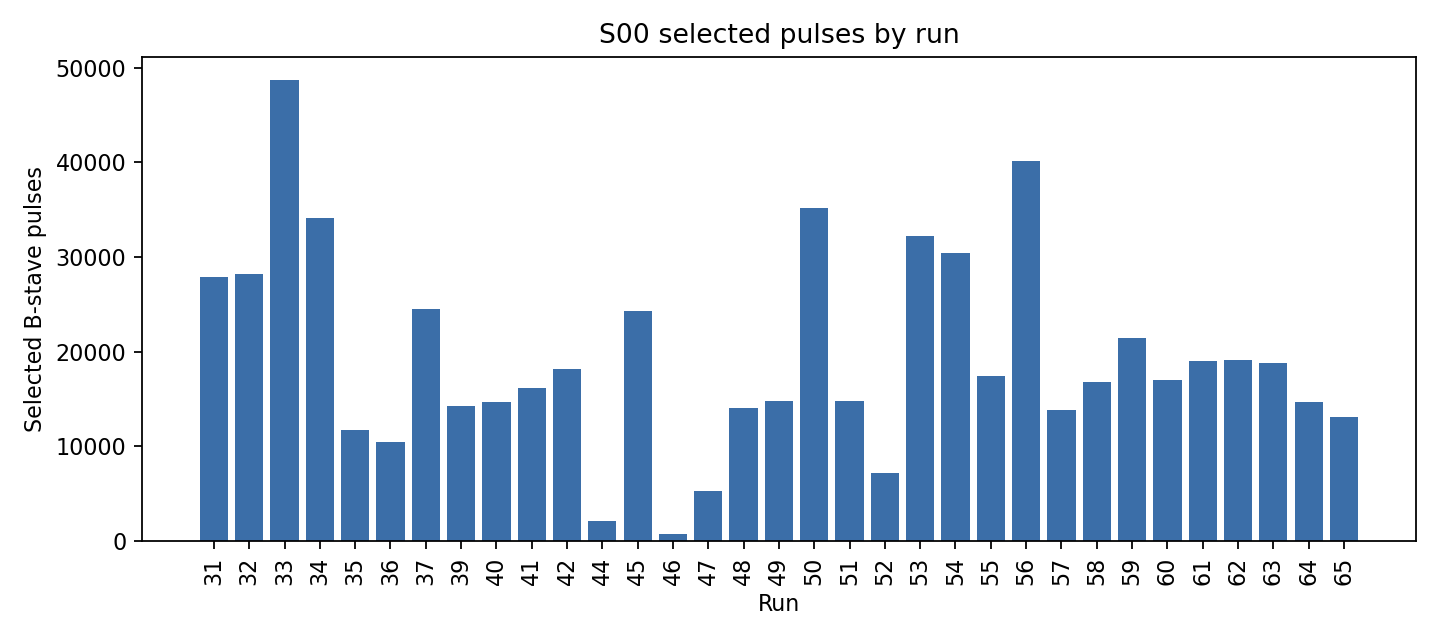
\includegraphics[width=0.48\textwidth]{../../reports/1780917628.449525.085b2dc0__s01b_s00_selected_table_manifest/fig_counts_by_run.png}
  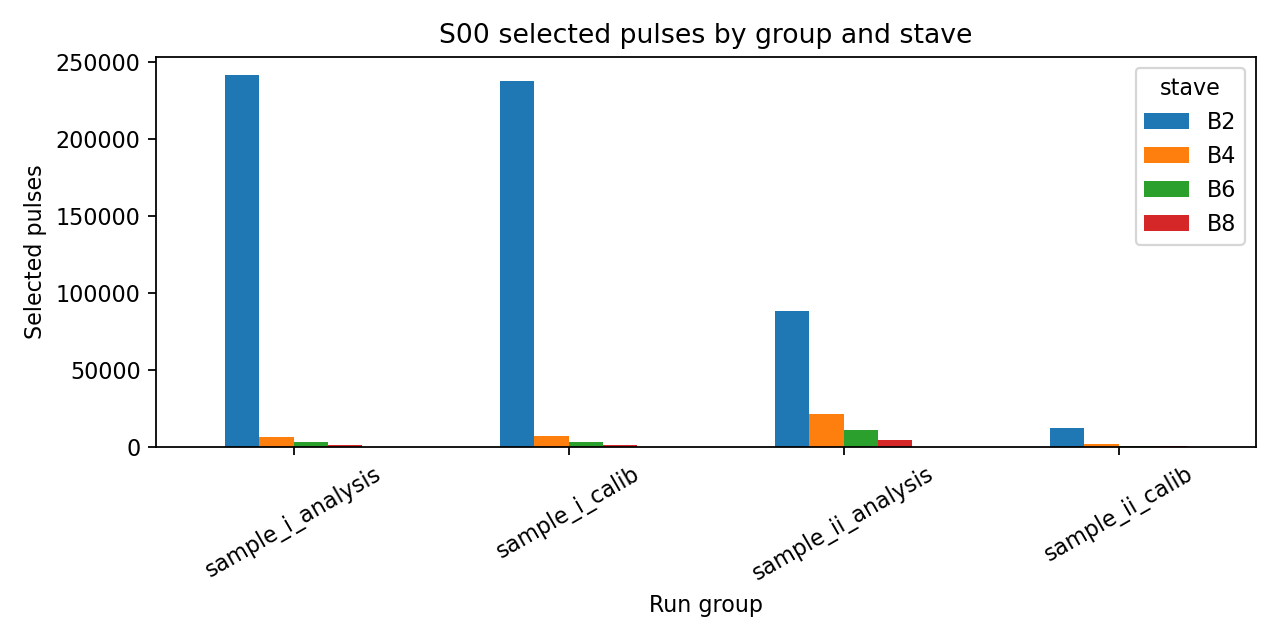
\includegraphics[width=0.48\textwidth]{../../reports/1780917628.449525.085b2dc0__s01b_s00_selected_table_manifest/fig_counts_by_group_stave.png}
  \caption{Selected-pulse count diagnostics from the S01b manifest.  Left:
  counts by run.  Right: group-by-stave composition after applying the physical
  even-channel convention.}
  \label{fig:s01b-counts}
\end{figure}

\section{Selection rule versus learned classifiers}
\label{sec:selection-ml}

The selection benchmark is intentionally asymmetric.  The traditional method is
the gate itself, Eq.~\ref{eq:s00-selection}; the machine-learning method is only
a sanity check that asks whether a classifier trained on summary features can
recover the same labels on held-out runs.  S00 and S01b used calibrated logistic
regression with amplitude, positive area, peak sample, and baseline features,
with runs 57 and 65 held out.  The model was well calibrated and nearly
perfect, but it was still inferior to the deterministic gate because the label
is the gate.

\begin{table}[H]
  \centering
  \small
  \caption{Run-held-out selection benchmark.  The deterministic threshold is
  the production method and wins.  The logistic model is retained only as a
  run-split sanity check.}
  \label{tab:selection-benchmark}
  \begin{tabular}{p{0.18\textwidth}p{0.28\textwidth}p{0.22\textwidth}p{0.22\textwidth}}
    \toprule
    Method family & Method & Metric & Value with 95\% CI \\
    \midrule
    Traditional & \(A>1000\) threshold & held-out accuracy & 1.000000 [1.000000, 1.000000] \\
    ML & calibrated logistic regression & held-out accuracy & 0.999796 [0.999491, 1.000000] \\
    \bottomrule
  \end{tabular}
\end{table}

The winner for selection is therefore the traditional deterministic threshold.
This conclusion is methodological as much as numerical: replacing an exact
definition by an approximate classifier would make the table less reproducible
without adding physics information.

\section{Amplitude-adaptive templates and \texorpdfstring{\(q_{\mathrm{template}}\)}{q-template}}
\label{sec:q-template}

After the selected table is fixed, S01 constructs an empirical pulse-shape
library.  Each selected waveform is baseline-subtracted, normalized by its peak
amplitude, and aligned on an 18-sample grid relative to the CFD20 crossing.
For stave \(s\) and amplitude bin \(k\), the traditional template is the
sample-wise median over calibration-run pulses,
\[
  T_{s,k,j} =
  \operatorname{median}_{e\in\mathcal{C}(s,k)} \tilde{y}_{e,j},
\]
where \(\tilde{y}\) denotes the aligned, amplitude-normalized waveform and
\(\mathcal{C}(s,k)\) contains calibration pulses in the stave and amplitude
bin.  Bins with fewer than 30 calibration pulses fall back to the stave-level
median.  The per-pulse template residual is
\[
  q_{\mathrm{template}}(e)
  =
  \left[
  \frac{1}{18}\sum_{j=0}^{17}
  \left(\tilde{y}_{e,j}-T_{s(e),k(e),j}\right)^2
  \right]^{1/2}.
  \label{eq:q-template}
\]
S01 writes \(q_{\mathrm{template}}\) for all \num{640737} selected pulses.
This scalar is not a truth label.  It is a compact residual describing how far
a pulse shape lies from its calibration-run stave/amplitude template.

\begin{figure}[H]
  \centering
  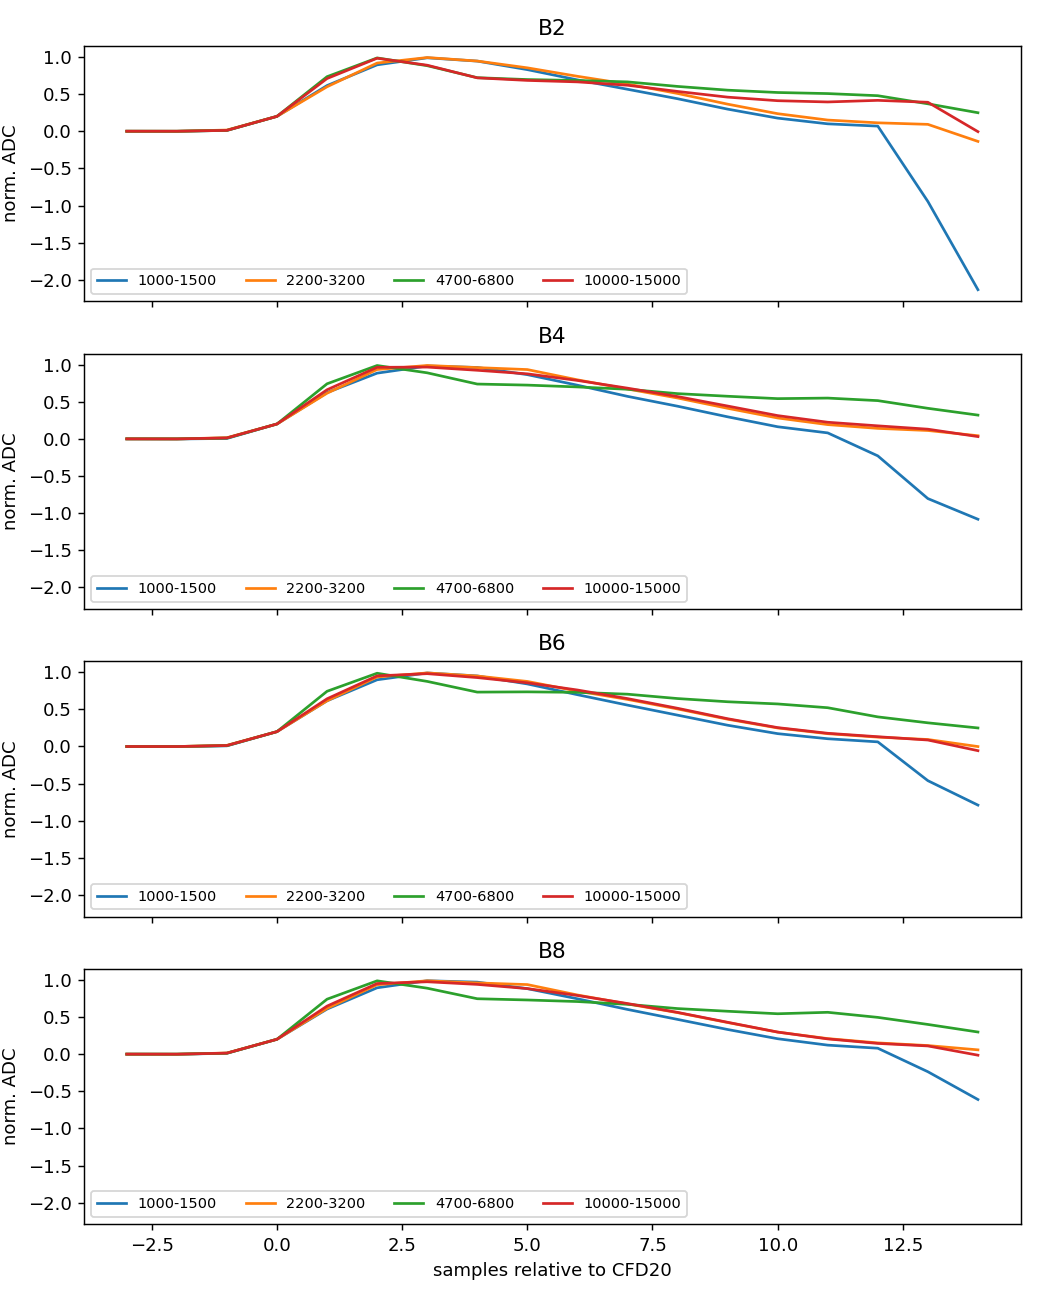
\includegraphics[width=0.48\textwidth]{../../reports/1780997954.15037.36463764__s01_full_dataset_templates/fig_template_library_examples.png}
  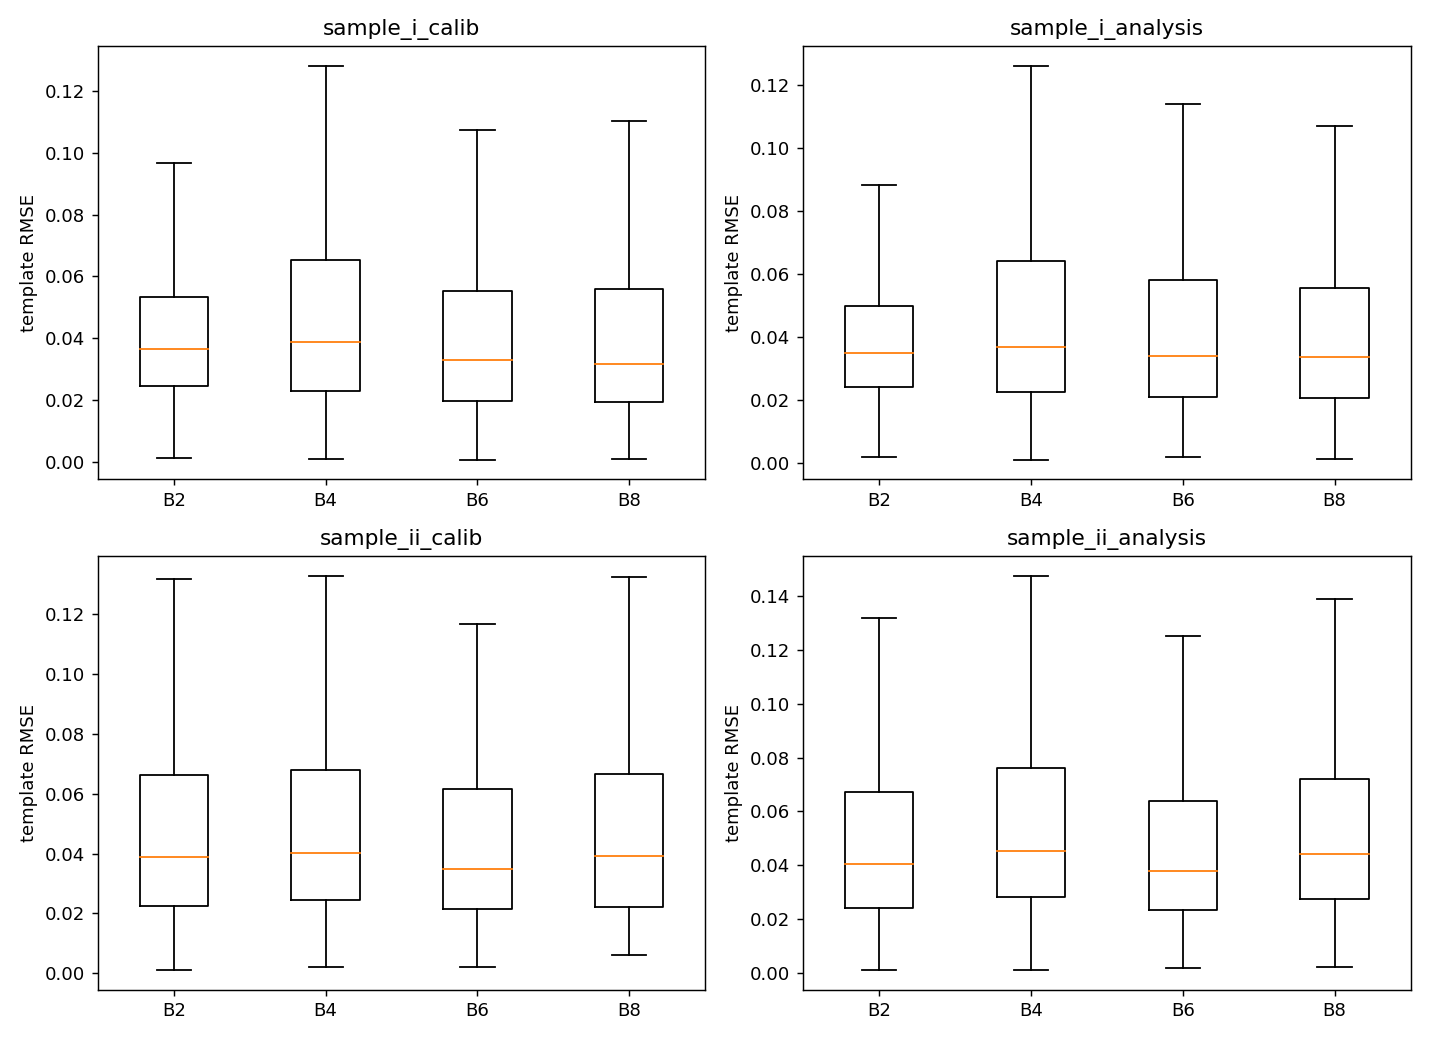
\includegraphics[width=0.48\textwidth]{../../reports/1780997954.15037.36463764__s01_full_dataset_templates/fig_q_template_by_group_stave.png}
  \caption{S01 amplitude-adaptive template outputs.  Left: examples from the
  empirical template library.  Right: \(q_{\mathrm{template}}\) distributions by
  group and stave for the full selected-pulse table.}
  \label{fig:s01-template-library}
\end{figure}

\section{Template benchmark: empirical median versus neural models}
\label{sec:template-benchmark}

S01 compared the empirical median template family with a fully connected
autoencoder trained only on calibration-run aligned waveforms.  Hyperparameters
were selected with grouped folds by run; the selected model used latent
dimension 8 and hidden dimension 32.  The benchmark metric was analysis-run
mean squared reconstruction residual on held-out analysis runs, with
run-bootstrap confidence intervals.  On this residual metric, the autoencoder
is the clear winner.

\begin{table}[H]
  \centering
  \small
  \caption{S01 held-out reconstruction benchmark for aligned, normalized pulse
  shapes.  Lower MSE is better.  Confidence intervals are 95\% run-bootstrap
  intervals over analysis runs.}
  \label{tab:s01-template-benchmark}
  \begin{tabular}{p{0.18\textwidth}p{0.32\textwidth}p{0.14\textwidth}p{0.26\textwidth}}
    \toprule
    Method family & Method & Metric & Value with 95\% CI \\
    \midrule
    Traditional & median stave/amplitude-bin template & MSE & 0.044414 [0.034249, 0.054782] \\
    NN & autoencoder, latent 8, hidden 32 & MSE & 0.002078 [0.001725, 0.002419] \\
    NN - traditional & difference & \(\Delta\)MSE & -0.042336 [-0.052421, -0.032381] \\
    \bottomrule
  \end{tabular}
\end{table}

The result is shown visually in Fig.~\ref{fig:s01-template-benchmark}.  The
neural model captures low-dimensional pulse-shape variation that is not
represented by fixed amplitude bins.  However, the S01 report correctly limits
the claim: the benchmark is reconstruction residual, not timing resolution,
particle identification, or absolute energy.  Downstream chapters evaluate
whether a lower waveform residual translates into a physics-facing observable.

\begin{figure}[H]
  \centering
  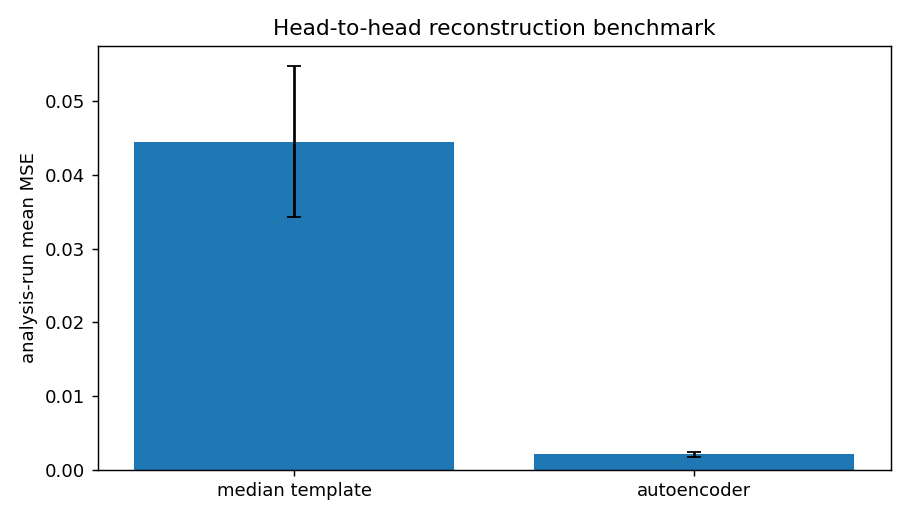
\includegraphics[width=0.72\textwidth]{../../reports/1780997954.15037.36463764__s01_full_dataset_templates/fig_template_vs_autoencoder_benchmark.png}
  \caption{S01 head-to-head reconstruction benchmark.  The autoencoder beats
  the empirical median template on held-out analysis-run MSE, but the result is
  interpreted as a shape-compression result rather than a physics calibration.}
  \label{fig:s01-template-benchmark}
\end{figure}

P10a tests a different neural architecture: a conditional MLP that maps stave
identity and log amplitude to an aligned normalized waveform template.  This
model improves a downstream phase-template timing metric but loses on the
primary \(q_{\mathrm{template}}\) MSE, and its shuffled-target control is a
warning that stave and amplitude alone do not define a stable held-out shape
generator.  For the reconstruction chapter, the empirical S01 template remains
the production definition of \(q_{\mathrm{template}}\).

\begin{table}[H]
  \centering
  \small
  \caption{P10a conditional-template stress test.  Lower is better for both
  metrics.  The primary \(q_{\mathrm{template}}\) metric favors the empirical
  amplitude-bin template; timing favors the conditional MLP but is treated as a
  downstream observation rather than a replacement for S01.}
  \label{tab:p10a-template-benchmark}
  \begin{tabular}{p{0.16\textwidth}p{0.27\textwidth}p{0.20\textwidth}p{0.27\textwidth}}
    \toprule
    Method family & Method & Metric & Value with 95\% CI \\
    \midrule
    Traditional & empirical amplitude-bin template & \(q\) MSE & 0.044414 [0.034222, 0.055344] \\
    NN & conditional MLP template & \(q\) MSE & 0.078062 [0.066158, 0.090569] \\
    NN - traditional & difference & \(\Delta q\) MSE & 0.033648 [0.027697, 0.041113] \\
    Traditional & empirical phase template & pairwise \(\sigma_{68}\) & 3.8306 ns [3.7325, 3.9344] \\
    NN & conditional MLP phase template & pairwise \(\sigma_{68}\) & 3.5789 ns [3.4857, 3.6801] \\
    NN - traditional & difference & \(\Delta\sigma_{68}\) & -0.2518 ns [-0.3781, -0.1331] \\
    \bottomrule
  \end{tabular}
\end{table}

\section{Amplitude-adaptive diagnostics in duplicate-readout closure}
\label{sec:p04c-closure}

The amplitude-adaptive template variables also appear in P04c, where the target
is the independent odd readout-side channel.  This is not an absolute energy
truth label, but it is a useful leakage-safe closure because the model inputs
use only the even physical-stave waveform and derived even-channel summaries;
run number, event number, and odd-channel samples are excluded.

P04c compares peak/integral baselines, fixed-bin template calibration,
adaptive-template scale, a stronger adaptive-template ridge, and a
histogram-gradient-boosted-tree regressor.  The strong traditional method is
the adaptive-template ridge, not the direct template scale.  Even so, the
gradient-boosted tree wins decisively on duplicate-readout closure.

\begin{table}[H]
  \centering
  \small
  \caption{P04c held-out duplicate-readout closure for runs 57 and 65.  Lower
  68th percentile absolute fractional error is better.  The winner is the
  gradient-boosted tree, but the interpretation is duplicate-readout closure,
  not absolute energy calibration.}
  \label{tab:p04c-closure}
  \begin{tabular}{p{0.14\textwidth}p{0.18\textwidth}p{0.34\textwidth}p{0.24\textwidth}}
    \toprule
    Target & Method family & Method & res68 with 95\% CI \\
    \midrule
    amplitude & Traditional & peak calibration & 0.1238 [0.1221, 0.1251] \\
    amplitude & Traditional & adaptive-template ridge & 0.0858 [0.0844, 0.0871] \\
    amplitude & ML & histogram-gradient-boosted trees & 0.00912 [0.00891, 0.00927] \\
    charge & Traditional & integral calibration & 0.1954 [0.1936, 0.1975] \\
    charge & Traditional & adaptive-template ridge & 0.1554 [0.1530, 0.1573] \\
    charge & ML & histogram-gradient-boosted trees & 0.0151 [0.0148, 0.0153] \\
    \bottomrule
  \end{tabular}
\end{table}

This closure result supports a broader pattern in the project.  Flexible ML
methods help when the task is a waveform-shape mapping to an independent
readout.  They should not be mistaken for detector truth when the target is
constructed from the same waveform or when no external energy/PID label exists.

\section{Systematic uncertainties and caveats}
\label{sec:data-systematics}

The dominant systematic risks in this chapter are not statistical fluctuations
of the selected count.  They are analysis-definition risks.

\begin{itemize}
  \item \textbf{Channel mapping.}  The selected table uses even raw channel
  blocks only.  Odd blocks are duplicate readout-side channels and belong in
  closure studies, not the production B-stave count.

  \item \textbf{Raw versus derived branches.}  The raw \texttt{HRDv} waveform
  rule is the selection authority.  Derived sorted \texttt{hrdMax} semantics do
  not reproduce the same gate and must not be used as a proxy for S00.

  \item \textbf{Processed-data availability.}  S01b found that the expected
  processed table was absent from the read-only data mirror in the sandbox.
  This is an infrastructure issue, not a physics discrepancy; the table is
  regenerated from raw ROOT and pinned by row count and checksum.

  \item \textbf{Template target semantics.}  \(q_{\mathrm{template}}\) is a
  reconstruction residual against a calibration-run empirical template.  It is
  not a truth label and not automatically a timing-quality, pile-up, or PID
  observable.

  \item \textbf{Run leakage.}  The quoted ML/NN comparisons use run-held-out or
  grouped-by-run validation.  This is essential because pulse shape, rate, and
  topology all vary by run and sample period.

  \item \textbf{Metric hierarchy.}  The autoencoder wins S01 reconstruction
  MSE, while the conditional MLP loses the primary P10a \(q\)-MSE but improves a
  timing metric.  The production choice therefore depends on the observable:
  empirical \(q_{\mathrm{template}}\) remains the transparent reconstruction
  variable; neural residuals are downstream candidates, not replacements for
  the selected-table definition.
\end{itemize}

\section{Chapter verdict}
\label{sec:data-verdict}

The selected data set is reproducible from raw ROOT: \num{640737} B-stave
pulses are recovered with zero count delta using the even-channel,
median-pedestal, \(A>1000\) ADC rule.  For selection, the traditional
deterministic threshold wins over calibrated logistic regression because it is
the exact definition and has held-out accuracy 1.000000.  For pulse-shape
reconstruction, the S01 autoencoder wins the held-out MSE benchmark over the
empirical amplitude-bin median template, with \(\Delta\mathrm{MSE}=-0.042336\)
and a 95\% CI entirely below zero.  For the production reconstruction record,
however, the empirical \(q_{\mathrm{template}}\) table remains the conservative
and interpretable artifact: it is tied to the exact S00 selected table, trained
only on calibration runs, and stress-tested against conditional neural
templates and duplicate-readout closure studies.
